
\chapter{Multiple Parton Interactions}
\label{chap:MultiplePartonInteractions}


By the fact that the hadrons are viewed as "bunches" of partons, it is likely that in the same hadron-hadron collision different couples of partons can undergo to a scattering. This phenomenon is known as \textit{Multiple Parton Interactions} (MPI) and it is related to the composite nature of the incoming hadrons. 
\\
So, it is clear that at some level these MPI have to exist, and they can become important in the description of the event; they can change the color topology of the colliding system as a whole.  
\\
In this scenario it is important to have a good understanding of the phenomenon. The aim of this section is to describe the basic concepts that are use to simulate MPI, for example in \texttt{Pythia} Monte Carlo event generator; than some focus is given to the free parameters we are going to tune in the following sections.

\section{Basic Concepts}
\label{sec:BasicConcepts}

The main hypothesis of the multiple interactions models is that: the QCD factorization theorem is true not only for the hard process but also for the other partons scatters.
\\
So, we can write:
\begin{equation}
	\frac{d\sigma_{\text{int}}}{dp_\perp}=\displaystyle\sum_{i,j,k,l}\displaystyle\int dx_1 \displaystyle\int dx_2 \displaystyle\int d\hat{t}\, f_i(x_1,Q^2)f_j(x_2,Q^2)\frac{d\hat{\sigma}_{ij\,\rightarrow\,kl}}{d\hat{t}}\delta\left( p_\perp^2-\frac{\hat{t}\hat{u}}{\hat{s}} \right) \quad .
	\label{eq:sigma_int1}
\end{equation}
This represent the interaction differential cross section for the hadron-hadron collisions, where $\frac{d\hat{\sigma}_{ij\,\rightarrow\,kl}}{d\hat{t}}$ is the differential cross section for QCD hard $2\ \rightarrow 2$ processes, this processes are the one reported in \tableRef{table:partonic_cross_sections}. 
\\
In \eqRef{eq:sigma_int1} we used the Mandelstam variables associated to the partonic system:
\begin{align}
	&\hat{s}=(p_1+p_2)^2=(p_3+p_4)^2=x_1x_2s\\
	&\hat{t}=(p_1-p_3)^2=(p_2-p_4)^2\\
	&\hat{u}=(p_1-p_4)^2=(p_2-p_3)^2
\end{align} 
where $p_1$, $p_2$ are the four-momenta of the incoming partons and $p_3$, $p_4$ the four-momenta of the outgoing partons. 

Note that in \eqRef{eq:sigma_int1} the jet cross section is twice as large $\sigma_{\text{jet}}=2\sigma_{\text{int}}$, because at first approximation each interaction gives rise to two jets.
\\
We assume also that the "hardness" of processes is defined by the $p_T$ scale of the interaction ($Q^2=p_T^2$).

%\begin{table}[!ht]
%	\centering
%	\begin{tabular}{l | c}\rule{0pt}{3ex} 
%	Process & Partonic cross section \rule{0pt}{3.5ex}\\   \hline\hline 
%	$q\,q'\ \rightarrow\ q\,q'$ & $\frac{4}{9}\frac{\hat{s}^2+\hat{u}^2}{\hat{t}^2}$\rule{0pt}{3.5ex}\\
%	$q\,q\ \rightarrow\ q\,q$ & $\frac{4}{9}\left(\frac{\hat{s}^2+\hat{u}^2}{\hat{t}^2}+\frac{\hat{s}^2+\hat{t}^2}{\hat{u}^2}\right) -\frac{8}{27}\frac{\hat{s}^2}{\hat{u}\hat{t}}$\rule{0pt}{3.5ex}\\
%	$q\,\overline{q}\ \rightarrow\ q'\,\overline{q}'$ & $\frac{4}{9}\frac{\hat{s}^2+\hat{u}^2}{\hat{t}^2}$\rule{0pt}{3.5ex}\\
%	$q\,\overline{q}\ \rightarrow\ q\,\overline{q}$ & $\frac{4}{9}\left(\frac{\hat{s}^2+\hat{u}^2}{\hat{t}^2}+\frac{\hat{t}^2+\hat{u}^2}{\hat{s}^2}\right) -\frac{8}{27}\frac{\hat{u}^2}{\hat{s}\hat{t}}$\rule{0pt}{3.5ex}\\
%	$q\,\overline{q}\ \rightarrow\ g\,g$ & $\frac{32}{27}\frac{\hat{t}^2+\hat{u}^2}{\hat{t}\hat{u}}-\frac{8}{3}\frac{\hat{t}^2+\hat{u}^2}{\hat{s}^2}$\rule{0pt}{3.5ex}\\
%	$g\,g\ \rightarrow\ q\,\overline{q}$ & $\frac{1}{6}\frac{\hat{t}^2+\hat{u}^2}{\hat{t}\hat{u}}-\frac{8}{3}\frac{\hat{t}^2+\hat{u}^2}{\hat{s}^2}$\rule{0pt}{3.5ex}\\
%	$g\,q\ \rightarrow\ g\,q$ & $-\frac{4}{9}\frac{\hat{s}^2+\hat{u}^2}{\hat{s}\hat{u}}-\frac{\hat{u}^2+\hat{s}^2}{\hat{t}^2}$\rule{0pt}{3.5ex}\\
%	$g\,g\ \rightarrow\ g\,g$ & $\frac{9}{2}\left( 3-\frac{\hat{t}\hat{u}}{\hat{s}^2} -\frac{\hat{s}\hat{u}}{\hat{t}^2} - \frac{\hat{s}\hat{t}}{\hat{u}^2} \right)$\rule{0pt}{3.5ex}
%	\end{tabular}
%	\caption{Parton-Parton differential cross sections ($2\ \rightarrow\ 2$ QCD process), can beh calculated in pQCD evaluating the matrix element for each process involving quark, antiquark and gluon.}
%	\label{table:partonic_cross_sections}
%\end{table}

\begin{table}[!ht]
	\centering	
	\begin{tabular}{| c | P{6cm} | c |}
	\hline
	Process & Amplitude & $\displaystyle\sum|\mathcal{M}|^2/(4\pi\alpha_s)^2$\\\hline\hline
	$qq'\,\rightarrow\,qq' $ & \scalebox{0.95}{\raisebox{-.5\height}{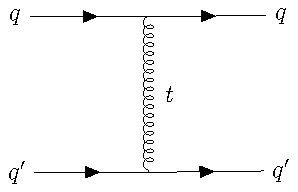
\includegraphics[width=2.5cm]{{img/DiagrammiPartonic/feynman_partonic_1.pdf}}}} & $\displaystyle{ \frac{4}{9}\frac{s^2+u^2}{t^2} }$\\\hline
	$qq\,\rightarrow\,qq $ & \scalebox{0.95}{\raisebox{-.5\height}{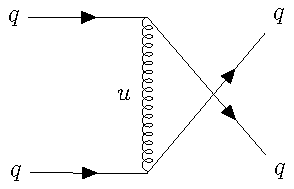
\includegraphics[width=2.5cm]{{img/DiagrammiPartonic/feynman_partonic_2.pdf}}\qquad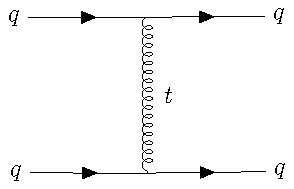
\includegraphics[width=2.5cm]{{img/DiagrammiPartonic/feynman_partonic_3.pdf}}}} & $\displaystyle{\frac{4}{9}\frac{s^2+u^2}{t^2} + \frac{4}{9}\frac{s^2+t^2}{u^2} - \frac{8}{27}\frac{s^2}{tu}}$\\\hline
	$q\overline{q}\,\rightarrow\,q'\overline{q'} $ & \scalebox{0.95}{\raisebox{-.5\height}{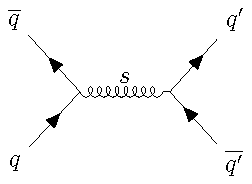
\includegraphics[width=2.5cm]{{img/DiagrammiPartonic/feynman_partonic_4.pdf}}}} & $\displaystyle{\frac{4}{9}\frac{t^2+u^2}{s^2}} $\\\hline
	$q\overline{q}\,\rightarrow\,q\overline{q} $ & \scalebox{0.95}{\raisebox{-.5\height}{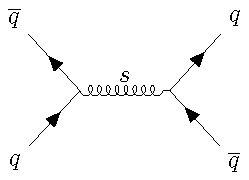
\includegraphics[width=2.5cm]{{img/DiagrammiPartonic/feynman_partonic_5.pdf}}\qquad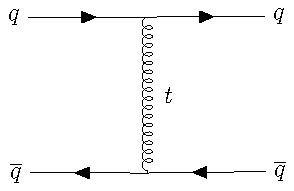
\includegraphics[width=2.5cm]{{img/DiagrammiPartonic/feynman_partonic_6.pdf}}}} & $\displaystyle{\frac{4}{9}\frac{s^2+u^2}{t^2} + \frac{4}{9}\frac{t^2+u^2}{s^2} - \frac{8}{27}\frac{u^2}{st}}$\\\hline
	$q\overline{q}\,\rightarrow\,gg $ & \scalebox{0.95}{\raisebox{0.0\height}{\vtop{\hbox{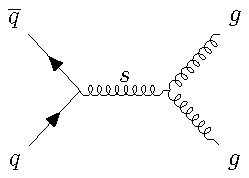
\includegraphics[width=2.5cm]{{img/DiagrammiPartonic/feynman_partonic_7.pdf}}\qquad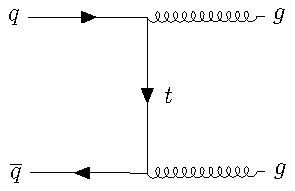
\includegraphics[width=2.5cm]{{img/DiagrammiPartonic/feynman_partonic_8.pdf}}}\begin{minipage}{4cm}{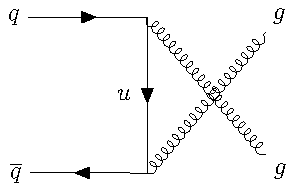
\includegraphics[width=2.5cm]{{img/DiagrammiPartonic/feynman_partonic_9.pdf}}}\end{minipage}}}} & $\displaystyle{\frac{32}{27}\frac{t^2+u^2}{tu}-\frac{8}{3}\frac{t^2+u^2}{s^2}} $\\\hline
	$gg\,\rightarrow\,q\overline{q} $ & \scalebox{0.95}{\raisebox{0.0\height}{\vtop{\hbox{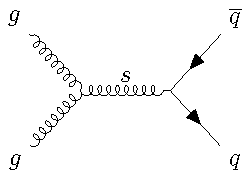
\includegraphics[width=2.5cm]{{img/DiagrammiPartonic/feynman_partonic_10.pdf}}\qquad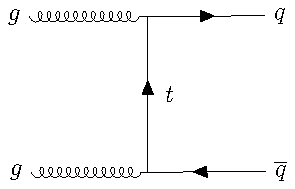
\includegraphics[width=2.5cm]{{img/DiagrammiPartonic/feynman_partonic_11.pdf}}}\begin{minipage}{4cm}{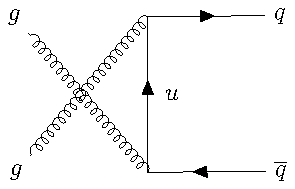
\includegraphics[width=2.5cm]{{img/DiagrammiPartonic/feynman_partonic_12.pdf}}}\end{minipage}}}} & $ \displaystyle{\frac{1}{6}\frac{t^2+u^2}{tu}-\frac{3}{8}\frac{t^2+u^2}{s^2}} $\\\hline
	$qg\,\rightarrow\,qg $ & \scalebox{0.95}{\raisebox{0.0\height}{\vtop{\hbox{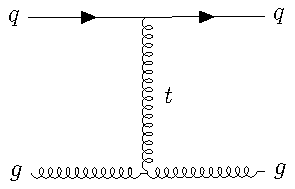
\includegraphics[width=2.5cm]{{img/DiagrammiPartonic/feynman_partonic_13.pdf}}\qquad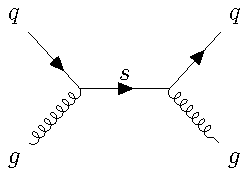
\includegraphics[width=2.5cm]{{img/DiagrammiPartonic/feynman_partonic_14.pdf}}}\begin{minipage}{4cm}{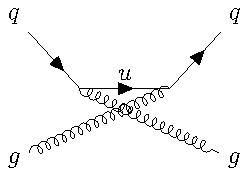
\includegraphics[width=2.5cm]{{img/DiagrammiPartonic/feynman_partonic_15.pdf}}}\end{minipage}}}} & $ \displaystyle{-\frac{4}{9}\frac{s^2+u^2}{su}+\frac{s^2+u^2}{t^2} }$\\\hline
	$gg\,\rightarrow\,gg $ & \scalebox{0.95}{\raisebox{0.1\height}{\vtop{\hbox{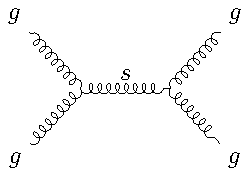
\includegraphics[width=2.5cm]{{img/DiagrammiPartonic/feynman_partonic_16.pdf}}\qquad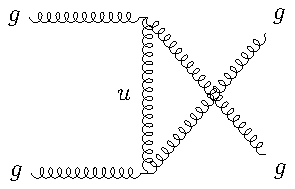
\includegraphics[width=2.5cm]{{img/DiagrammiPartonic/feynman_partonic_17.pdf}}}\hbox{\raisebox{0.1\height}{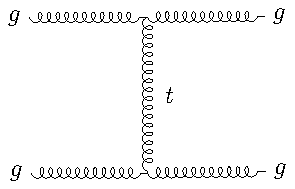
\includegraphics[width=2.5cm]{{img/DiagrammiPartonic/feynman_partonic_18.pdf}}\qquad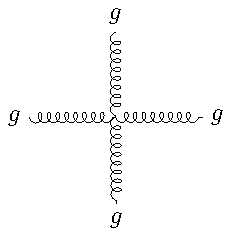
\includegraphics[width=2.5cm]{{img/DiagrammiPartonic/feynman_partonic_19.pdf}}}}}}} & $ \displaystyle{\frac{9}{2}\left( 3-\frac{tu}{s^2}-\frac{su}{t^2}-\frac{st}{u^2}\right)} $\\\hline
	\end{tabular}
	\caption{Parton-Parton differential cross sections ($2\ \rightarrow\ 2$ QCD process), can beh calculated in pQCD evaluating the matrix element for each process involving quark, antiquark and gluon. Table from \cite{SIEGERTthesis}}
	\label{table:partonic_cross_sections}
\end{table}

%\begin{table}[!ht]
%	\centering
%	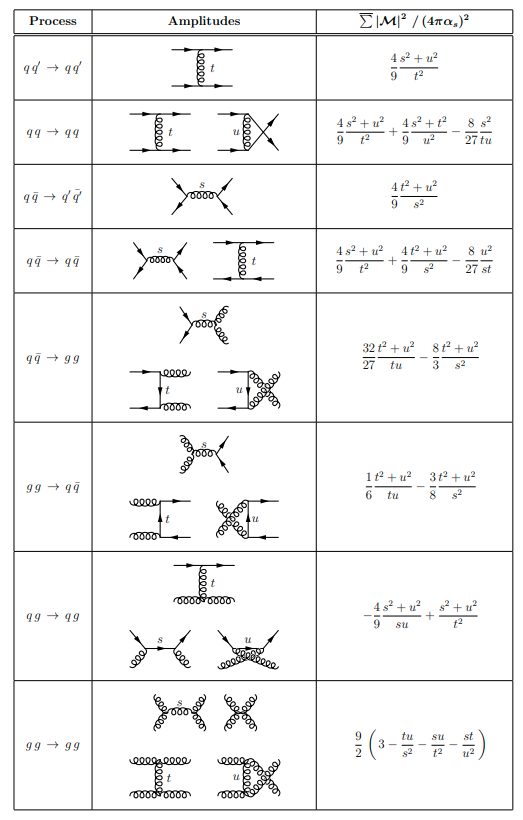
\includegraphics[width=0.8\textwidth]{{img/Table_cross_sections.png}}
%	\caption{Parton-Parton differential cross sections ($2\ \rightarrow\ 2$ QCD process), can beh calculated in pQCD evaluating the matrix element for each process involving quark, antiquark and gluon. Table from \cite{SIEGERTthesis}}
%	\label{table:partonic_cross_sections}
%\end{table}

\noindent As you can see from the formulae in \tableRef{table:partonic_cross_sections}
at small scattering angles, for $t\,\rightarrow\,0$,  the t-channel gluon exchange processes $qq'\,\rightarrow\,qq'$, $qg\,\rightarrow\,qg$ and $gg\,\rightarrow\,gg$ dominate the full matrix element. For scatterings that are soft relative to $\hat{s}$, $|\hat{t}|\ll \hat{s}$, we can approximate $|\hat{t}|$ as:
\begin{equation}
	p_T^2=\frac{\hat{t}\hat{u}}{\hat{s}} = \frac{\hat{t}(-\hat{s}-\hat{t})}{\hat{s}} \approx |\hat{t}|\quad ,
\end{equation}
in this limit, the only differences between quark and gluon cross sections are the color factors
\begin{equation}
	\hat{\sigma}_{gg}:\hat{\sigma}_{qg}:\hat{\sigma}_{qq}=\frac{9}{4}:1:\frac{4}{9}\quad .
\end{equation}
So, the \eqRef{eq:sigma_int1} can be rewritten like
\begin{equation}
	\frac{d\sigma_{int}}{dp_T^2}\approx\int\int\frac{dx_1}{x_1}\,\frac{dx_2}{x_2}\,F(x_1,p_T^2)\,F(x_2,p_T^2)\frac{d\hat{\sigma}_{2\,\rightarrow\,2}}{dp_T^2}\quad ,
	\label{eq:sigma_int2}
\end{equation}
whit:
	\begin{gather}
		\frac{d\hat{\sigma}_{2\,\rightarrow\,2}}{dp_T^2} = \frac{8\pi\alpha_s^2(p_T^2)}{9p_T^4}\quad ;\\
		F(x,Q^2)=\displaystyle\sum_q\left( x\,q(x,Q^2) + x\,\overline{q}(x,Q^2) \right) + \frac{9}{4}\,x\,g(x,Q^2)\quad .
	\end{gather}
Now, we can integrate the \eqRef{eq:sigma_int2}:
\begin{equation}
	\sigma_{int}(p_{T\,min})= \displaystyle\int_{ p_{T\,min}^2}^{(\sqrt{s}/2)^2}\frac{d\hat{\sigma}_{2\,\rightarrow\,2}}{dp_T^2}\,dp_T^2\propto \frac{1}{p_{T\,min}^2}\  \xrightarrow{\ \ p_{T\,min}\,\rightarrow\, 0 \ }\ \ \infty
	\label{eq:interaction_crossSection}
\end{equation}

\begin{figure}[!ht]
	\centering
	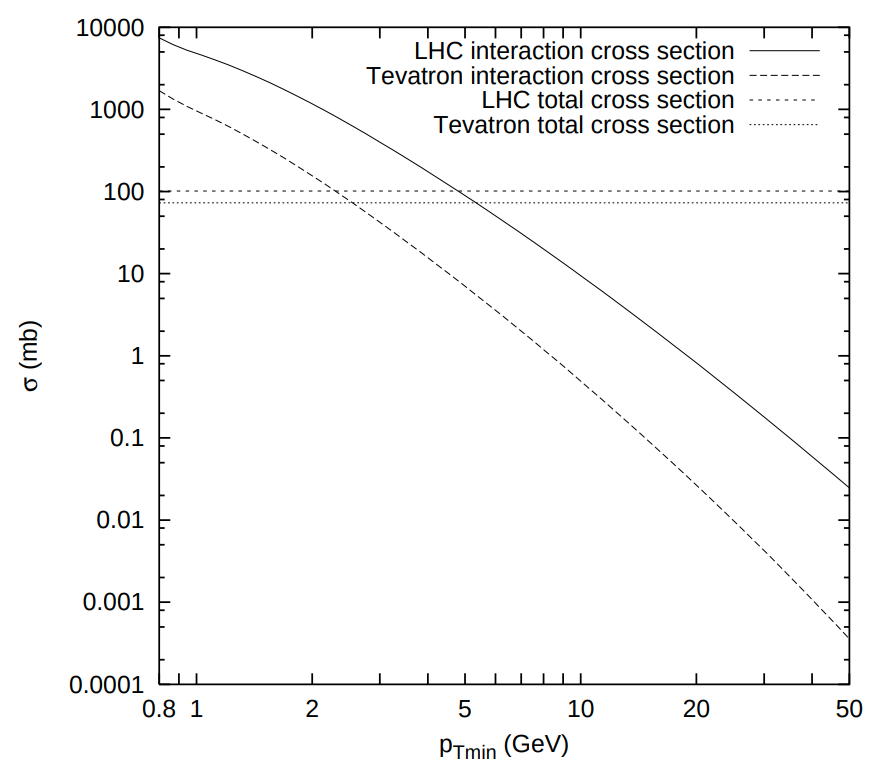
\includegraphics[width=12cm]{{img/CrossSection_Tot.png}}
	\caption{This figure shows the interaction cross section ($\sigma_{\text{int}}$) at Tevatron ($p\overline{p}$, $\sqrt{s}=1.8\ \mathrm{TeV}$) and at LHC ($pp$, $\sqrt{s}=14\ \mathrm{TeV}$). The flat lines are the corresponding values for the total cross section. The interaction cross section that arise from \eqRef{eq:interaction_crossSection} is divergent for $p_{T\,min}\,\rightarrow\,0$ in reality a dumping of this divergence is expected due to the color screening effect.}
	\label{fig:CrossSection_Tot}
\end{figure}

\noindent The total cross section is divergent in the limit $p_T\,\rightarrow\,0$, this divergence is shown in \figRef{fig:CrossSection_Tot}. Due to this divergence the total interaction cross section at some $p_{T}$ scale can exceed the total proton-proton cross section.
\\
To understand this paradox should be noted that the interaction cross section described in \eqRef{eq:interaction_crossSection} is related to the interaction probability between two partons and counts the number of interactions, while the total proton-proton cross section $\sigma_{pp}$ counts the number of events. For example, an event (a proton-proton collision) in which two partons interact counts once in the total cross section and twice in the interaction cross section.
\\
So, the ratio between this two quantities is perfectly allowed to be larger than unity, we can write it down as:
\begin{equation}
	\frac{\sigma_{int}(p_{T\,min})}{\sigma_{tot}}=\langle n \rangle (p_{T\,min})\quad .
\end{equation}
Furthermore, we have to consider the \textit{screening effect}: in fact the incoming hadrons are color singlet objects. Therefore, when the $p_T$ of an exchanged gluon is small, and so the associated wavelength large, this gluon cannot longer resolve the color charges and the effective coupling is decreased, this screening set a cutoff in the divergence. The screening effect is schematically shown in \figRef{fig:ScreeningEffect}.

\begin{figure}[!ht]
	\centering
	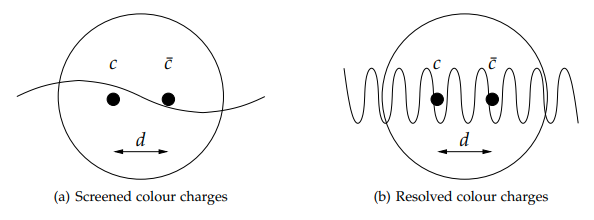
\includegraphics[width=0.7\textwidth]{{img/ScreeningEffect.png}}
	\caption{A picture of the screening effect. The left figure show two color charge that are not resolved by the gluon in fact the wave length is greater than the spatial separation, $d$, of the two charges. So resolution of the probe is not enough to discriminate the color charges. While on the right figure the two charges are very well distinct.}
	\label{fig:ScreeningEffect}
\end{figure}

\noindent This cutoff is associated with color screening distance i.e. the average size of the region within the  compensation of color charge occurs.
This cutoff is then introduced in the factor as
\begin{equation}
	\frac{\alpha_s^2\,(p_{T0}^2+p_{T}^2)}{\alpha_s^2\,(p_T^2)}\,\frac{p_T^4}{(p_{T0}^2+p_T^2)^2}\quad .
\end{equation}
This factor contains the phenomenological regularization of the divergence, with the factor $p_{T0}$ that have to be tuned to data. 
\\
Now the interaction cross section is smoothly regularized and therefore finite.
\\
To be notice that: parameter $p_{T0}$ do not have to be energy-independent, but since the energy is related with the sensibility of our probe, higher energy is related with the capacity of probing PDF to lower x values (as discussed previously, see \figRef{fig:NNPDF31}) and in this low x region the number of partons rapidly increases. So, the partons are closer packed in this regions and as a consequence the color screening distance decrease.
\\
The number of partons is related to $x$ with a power low so, it is likely to have a dependence of the same form for $p_{T0}$ respect to the center-of-mass energy
\begin{equation}
	p_{T0}(\sqrt{s})=p_{T0}^{ref} \,\left( \frac{\sqrt{s}}{E_{CM}^{ref}} \right)^{E_{CM}^{pow}}\quad .
\end{equation}
	
	
In the next section we are going to discuss how this and other effects fit into the Monte Carlo generator \texttt{pythia8}.	
	
\section{\texttt{Pythia8} Monte Carlo events generator}	

\texttt{Pythia}8 is a standard tool for the simulation of events in high energy collisions. \texttt{Pythia} contains the evolution from a few-body system to a complex multiparticles final state.

\subsection{Parton Shower}

 In \texttt{Pythia}8 all the contributions from Initial State Radiation (ISR), Final State Radiation (FSR) and Multi Parton Interactions (MPI) are interleaved into a single common sequence of decreasing $p_T$. 
\\
The parton shower has been described in the previously section. The solution to the DGLAP equation is given putting \eqRef{eq:FSR1} and \eqRef{eq:ISR1} in \eqRef{eq:sudakovFormFactor} for the ISR and the FSR by a Sudakov form factor that is related to the no emission probability in the $p_T$-evolution. 
\\
The evolution variables for ISR and FSR are defined starting from the virtuality ($Q^2$) of the emission:
\begin{equation}
	p_T^2=\left\{\begin{aligned}
		&(1-z)Q^2 && ISR\\
		&z(1-z)Q^2 && FSR
	\end{aligned}\right.\quad,
	\label{eq:partonShowerEvolutionVariables}
\end{equation}
so, in the two cases: for the FSR $Q^2_{FSR}=(p^2-m_0^2)$ in fact a time-like virtuality ($p^2>0$) is implicated, while for the ISR we have $Q^2_{ISR}=(-p^2+m_0^2)$ with a space-like virtuality ($p^2<0$). In both case $Q^2$ values are positive defined. Than the actual strong of the radiation is set by the choices of $\alpha_{s\,ISR}$ and $\alpha_{s\,FSR}$ values.

\subsection{Multiple Parton Interactions in \texttt{Pythia}}

The MPI, as said before, are also generated in a decreasing $p_T$ sequence. So the hardest MPI is generated first. Than we can write the probability for an interaction, $i$, to occur at a scale $p_T$ using a Sudakov-type expression (as we have done for the ISR and the FSR):
\begin{equation}
	\frac{d\mathcal{P}_{MPI}}{dp_T}=\frac{1}{\sigma_{ND}}\frac{d\sigma_{2\,\rightarrow\,2}}{dp_T}\ \exp\left( -\displaystyle\int_{p_T}^{p_T\,i-1} \frac{1}{\sigma_{ND}}\frac{d\sigma_{2\,\rightarrow\,2}}{dp_T'}\,dp_T' \right)\quad .
\end{equation}


\subsection{Momentum and flavour conservation}

One problem is to achieve momentum conservation, so we need to take into account the modification in the PDF by the $i-1$ interaction. To do that in \texttt{Pythia} the PDF are rescaled to the remaining available $x$ range, adjusting their normalization.
\\
We need to take into account the momentum fraction $x_i$ removed from the hadron remnant by the $i-th$ interaction. This is done evaluating PDF not at $x_i$ but at a rescaled value
\begin{equation}
	x_i'=\frac{x_i}{X} \qquad \ \text{with }\ \ X=1-\sum_{j=1}^{i-1}x_j\quad .
\end{equation}
So, using these quantities, we can rewrite our PDFs as:
\begin{equation}
	f_i(x,Q^2)\ \longrightarrow\ \frac{1}{X}f_0\left(\frac{x}{X}\right)\quad ,
\end{equation}
where $f_0$ is the original one-parton inclusive PDFs.
\\
Now, requiring also the flavour conservation and taking into account the number of valence and/or sea quarks involved in the preceding MPI. We have now the full forms of the PDFs used for the $i-th$ MPI:
\begin{align}
f_i(x,Q^2) =&  \frac{N_{fv}}{N_{fv0}}\frac{1}{X} f_{v0}\left( \frac{x}{X},Q^2 \right) + \frac{a}{X}f_{s0}\left( \frac{x}{X},Q^2 \right)+\displaystyle\sum_j \frac{1}{X} f_{c_j0}\left( \frac{x}{X},Q^2 \right) \quad,\\
g_i(x,Q^2) =& \frac{a}{X}g_0\left( \frac{x}{X},Q^2 \right)\quad, 
\end{align}
where: 
\begin{itemize}
	\item $f_i(x,Q^2)$ $(g_i(x,Q^2))$ are the squeezed PDFs for quarks (gluons);
	\item $N_{fv}$ the number of remaining valence quarks of the given flavour;
	\item $N_{fv0}$ the number of original valence quarks of the given flavour (for the proton we have $N_u=2$, $N_d=1$);
	\item $f_{s0}$ the sea-quark PDF;
	\item $f_{cj}$ the companion PDF, this arise from the splitting $g\,\rightarrow\,q\overline{q}$ and a quark $j$ is kicked out.
\end{itemize}
The factor $a$ is defined to satisfy the total momentum sum rule.

\subsection{Impact Parameter Dependence}

The simplest hypothesis for the multiple interaction simulation, it is to assume the same initial state for all hadron collisions without dependencies on the impact parameter. 
\\
The more realistic scenario it is to include the possibility that each collision could be characterized by a different impact parameter $b$, where a small $b$ value correspond to a large overlap between the two hadrons this is related to the probability of parton-parton interaction to take place.
\\
To include the impact parameter dependence on the collision, it is necessary to make some assumption on the matter distribution inside the proton. A possibility is to assume a spherically symmetric distribution inside an hadron at rest $\rho(\mathbf{x})\,d^3x=\rho(r)\,d^3x$. A Gaussian ansatz is the most simple choice but it appears to lead to a narrow multiplicity distribution and a too little pedestal effect. So the coiche is a double Gaussian:
\begin{equation}
	\rho(r) \propto \frac{1-\beta}{a_1^3}\exp\left\{-\frac{r^2}{a_1^2}\right\}+\frac{\beta}{a_2^3}\exp\left\{ -\frac{r^2}{a_2^2} \right\}\quad,
	\label{eq:matterDistribution}
\end{equation}
where a fraction $\beta$ of matter is contained in a radius $a_2$, and the rest in a larger radius $a_1$.

\medskip

Now, for a given matter distribution $\rho(r)$,  the time-integrated overlap function of the incoming hadrons during the collision is given by:
\begin{equation}
	\mathcal{O}(b)=\displaystyle\int dt \displaystyle\int d^3x\,\rho(x,y,z)\,\rho(x+b,y,z+t)\quad.
	\label{eq:overlappingFunction}
\end{equation} 
Assuming the matter distribution function in \eqRef{eq:matterDistribution} and inserting it into \eqRef{eq:overlappingFunction} we get  the following expression.
\begin{equation}
\small{
	\mathcal{O}(b)\propto \frac{(1-\beta)^2}{2a_1^2}\exp\left\{-\frac{b^2}{2a_1^2}\right\}+\frac{2\beta(1-\beta)}{a_1^2+a_2^2}\exp\left\{ -\frac{b^2}{a_1^2+a_2^2} \right\}+\frac{\beta^2}{2a_2^2}\exp\left\{-\frac{b^2}{2a_2^2}\right\}
	}
\end{equation}
this is useful to quantify the effect of overlapping protons.
The larger is $\mathcal{O}(b)$ the more probable are parton-parton scatters between the incoming protons $\langle \widetilde{n} \rangle\propto \mathcal{O}(b)$.

\medskip

So, these assumption change the so-far Poissonian nature of the framework\footnote{the Poissonian distribution, in \eqRef{eq:poisson} describe the probability of having $n$ interactions at each impact parameter. If the matter distribution have an infinite tail (like our in \eqRef{eq:matterDistribution}) events may be obtained with arbitrarily large b values. This can be a problem for the definition of the total hadron-hadron cross section}
\begin{equation}
\mathcal{P}(\widetilde{n})=
	\left\langle \widetilde{n}\right\rangle ^{\widetilde{n}}\ \frac{e^{-\langle\widetilde{n}\rangle}}{\widetilde{n}!}
	\label{eq:poisson}
\end{equation}
Now the request that at least one parton interactions in the hadron-hadron collision, ensures that we get a finite total cross section. So the probability that an event is produced by two hadrons scattering with impact parameter $b$:
\begin{equation}
	\mathcal{P}_{\text{int}}= \displaystyle\sum_{\widetilde{n}=1}^\infty\mathcal{P}_{\widetilde{n}(b)}=1-\mathcal{P}_0=1-e^{-\langle \widetilde{n}(b) \rangle}=1-e^{-k\mathcal{O}(b)}
\end{equation}
So we have now that the number of interaction per event is give by (for impact parameter $b$):
\begin{equation}
	\langle n(b) \rangle=\frac{\langle \widetilde{n}(b) \rangle}{\mathcal{P}_{\text{int}}}
\end{equation}
so, this have modified the probability distribution of interactions number from a Poissonian to a narrower one at each $b$ fixed.

\subsection{Parton rescattering}

It is not necessary that the partons undergoing to a MPI are a different partons couple from the one scattered before. As shown in \figRef{fig:Rescattering} MPI can also arise when a parton scatters more than once against partons from the other beam, this is call \textit{parton rescattering}. 

\begin{figure}[!ht]
	\centering
	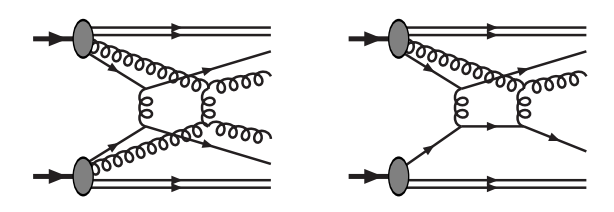
\includegraphics[width=12cm]{{img/Rescattering.png}}
	\caption{Add caption}
	\label{fig:Rescattering}
\end{figure}

We can have 3 type of MPI:
\begin{enumerate}
	\item No ones of the partons that enter in the second scattering undergoes to another scatter before
	\item Only one of the two partons have alredy been scattered
	\item Both the partons have alredy been scattered before.
\end{enumerate}
The second and the third are the rescatters the overall influence of rescatters in proton-proton interactions was estimated to be small respect to the first case with distinct $2\,\rightarrow\,2$  scatters. 

The simulation of parton rescatters start from the evaluation of the parton density as:
\begin{equation}
	f(x,Q^2)\ \  \longrightarrow\! \underbrace{\phantom{\Bigg(} f_{\text{rescaled}}(x,Q^2)}_{\text{hadron remnant}}+\underbrace{\displaystyle\sum_n \,\delta(x-x_n)}_{\text{scattered parton(s)}}
\end{equation} 

The $\delta$ take into account the scattered partons that have a fixed momentum fraction $x_n$. While the hadron remnant is still described by a continuous momentum density, rescaled to achieve momentum conservation:
\begin{equation}	\displaystyle\int_0^1 \bigg( f_{\text{rescaled}}(x,Q^2) +\displaystyle\sum_n \,\delta(x-x_n) \bigg)dx=1
\end{equation}

\subsection{Interleaving of Multiple Interaction and Parton Shower}

As discussed above the MPI are simulated in \texttt{Pythia} following a decreasing $p_T$ evolution.
So we have that the total probability is given from the composition of the various contributions:
\begin{align}
	\frac{d\mathcal{P}}{dp_T}=&\left( \frac{d\mathcal{P}_{MPI}}{dp_T}+\displaystyle\sum\frac{d\mathcal{P}_{ISR}}{dp_T}+\displaystyle\sum\frac{d\mathcal{P}_{FSR}}{dp_T} \right) \nonumber \times\\ 
	&\times\exp\left\{ -\displaystyle\int_{p_T}^{p_T\,i-1} \left( \frac{d\mathcal{P}_{MPI}}{dp_T'}+\displaystyle\sum\frac{d\mathcal{P}_{ISR}}{dp_T'}+\displaystyle\sum\frac{d\mathcal{P}_{FSR}}{dp_T'} \right)\,dp_T' \right\}
	\label{eq:common_pT_sequence}
\end{align}

\begin{figure}[!ht]
	\centering
	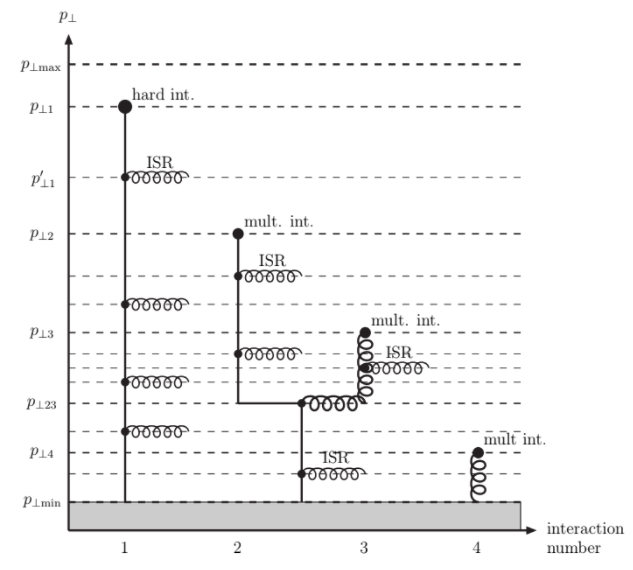
\includegraphics[width=12cm]{{img/PartonShower.png}}
	\caption{add caption}
	\label{fig:PartonShower}
\end{figure}

In \figRef{fig:PartonShower} are shown 4 parton-parton interactions with their associated showers (ISR and FSR). The downward evolution correspond to read the graph from top to bottom. The first hard interaction occur at a scale $p_T=p_{T1}$ while the following ones at lower scales $p_{T2}$, $p_{T3}$, $p_{T4}$. Each interaction is associated with is radiation the first one occurs at $p_T=p_{T1}'$.
The scatterings that occur at $p_{T2}$ and $p_{T3}$ are originating from the same mother parton. 

This diagram is related to one of the two hadrons. The full event can be illustrated if a similar diagram is drawn for the other hadron and connected to the full black circles.

\subsection{Beam Beam Remnants and primordial $k_T$}

What is left after that the evolution is end? the evolution in $p_T$ can create an arbitrary complicate final state. 

This final state contains contributions from the scattered and unscattered partons that don't enter the $p_T$ evolution. The last are the so called Beam Beam Remnants (BBR). 
BBR take into account the number of valence quark remaining and the number of sea quark required for the overall flavour conservation.

To ensure momentum conservation the BBR have to take all the remaining longitudinal momentum that is not extracted by the MPI initiators.

\subsubsection*{Primordial $k_T$}

We have considered only the longitudinal momentum. in a real scenario partons inside the hadrons are fermions so are expected to have a non zero initial transverse momentum arising from the Fermi motion inside the incoming hadrons. This is denoted as "Primordial $k_T$" this is different from the transverse momentum derived from DGLAP shower evolution or from the hard interaction.

\bigskip

Based on Fermi motion alone, one would expect a value of the primordial $k_T$ is estimate as: 
\begin{equation}
	k_T\simeq\frac{\hbar}{r_p}\approx\frac{0.2\ \mathrm{GeV\cdot fm}}{0.7\ \mathrm{fm}}\approx0.3\ \mathrm{GeV}
\label{eq:PrimordialKT}
\end{equation}
but for example to reproduce the data for the the $p_T$ distributions of $Z$ bosons produced in hadron–hadron collisions, one need a larger contribution. This phenomenon has not a satisfactory explanation. Until an explanation is found the idea is to consider a effective primordial $k_T$ for the initiators larger than the one in \eqRef{eq:PrimordialKT}.

In \texttt{Pythia} the primordial kT is assigned to initiators sampling a Gaussian distributions for $p_x$ and $p_y$ independently with variable width $\sigma$

\begin{equation}
	\sigma(Q,\widehat{m})=\frac{Q_{1/2}\,\sigma_{\text{soft}}+Q\,\sigma_{\text{soft}}}{Q_{1/2}+Q}\,\frac{\widehat{m}}{\widehat{m}_{1/2}+\widehat{m}}
\end{equation}
 
Where $Q$ is the hard-process renormalization scale for the main hard process and the $p_T$ scale for subsequent MPI. $\sigma_{\text{soft}}$, $\sigma_{\text{hard}}$ are the minimum and maximum width, $\widehat{m}$ is the invariant mass, while $Q_{1/2}$ and $\widehat{m}_{1/2}$ the halfway values between the two extremes.

\subsection{Color Reconnection and Hadronization }

The last important step at parton level is the color reconnection. Color reconnection is motivated by that MPI leads to different color strings. In the previous step the planar limit of the QCD was assumed where $N_c\rightarrow\infty$. Now, moving to real case where $N_c=3$ all this strings that can be overlapped in physical space can be reconnected. The basic idea is to reconnect strings in order to reduce the total string length; and thus the potential energy.

In \textsc{pythia8} the reconnection is performed giving to each system a probability to reconnect given by:
\begin{equation}
	\mathcal{P}_{\text{rec}}=\frac{p_{T\,\text{rec}}^2}{\left(p_{T\,\text{rec}}^2 + p_T^2\right)} \qquad\quad p_{T\,\text{rec}}=R\times p_{T\,0}
\end{equation} 
the \texttt{ColorReconnection:range} $R$ is a user-tunable parameter while $p_{T\,0}$ is the same parameter defined in MPI simulation.

Whit this definition for the probability it is clear that system with low $p_T$ are more likely that can reconnect to other, this idea find is justification in the fact that at low $p_T$ value correspond a larger spatial extension and so these strings have more chance to overlap with other and so to reconnect.

The hadronization takes all these partons (color strings) and transform it in a set of color-neutral hadrons. Hadronization is based solely on the \textit{Lund string fragmentation model} \cite{ANDERSSON198331, Sjostrand:1984ic}. 

Lund model basic idea is to break the color line and to reduce the total string length the string is representative of the potential
\begin{equation}
	V(r)=-\frac{a}{r}+\kappa r \qquad\qquad \text{with}\quad \kappa\approx1\ \mathrm{GeV/fm}
\end{equation}
where $\kappa$ is the string tension.  This potential is a combination of an attractive (Coulomb) potential ad a linear potential that phenomenologically include quarks confinement. The linear potential is the dominating part at increasing distance values, so the energy increase with distance. 

The simplest case is the one in \figRef{fig:StringBreakings}: The $q\overline{q}$ system evolves in space increasing the string length at some point the distance is to large and is convenient to break the string into two strings.

\begin{figure}[!ht]
	\centering
	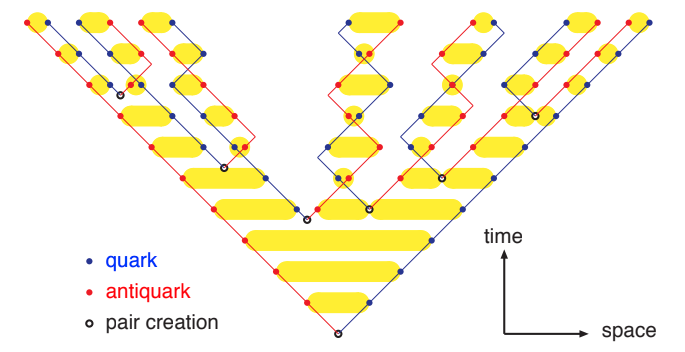
\includegraphics[width=12cm]{{img/StringBreakings.png}}
	\caption{ADD}
	\label{fig:StringBreakings}
\end{figure}

%So the hadronization try to reduce the string length.
%\begin{equation}
%	V(r)=-\frac{a}{r}+\kappa r \qquad\qquad \text{with}\quad \kappa\approx1\ \mathrm{GeV/fm}
%\end{equation}
The hadronization step confines the quark into hadrons, than hadrons can undergoes to hadron rescattering and decay. These are the hadrons that are revealed by the detector.

\section{\textsc{pythia} summary}

Tu summarize \textsc{pythia8} is able to simulate an high energy hadron-hadron collision. The evolution of the system is simulated in a common decreasing-$p_T$ sequence the master formula for the evolution is written in \eqRef{eq:common_pT_sequence}. 

This evolution start from an hard scale that is the scale of the main parton hard scattering that is described by a fixed ME calculation, \textsc{pythia} can be interfaced with external frameworks for the ME step as \textsc{powheg} and \textsc{mad-graph5 amc@nlo}. Then the parton shower is started with the simulation of ISR, FSR and MPI also the parton rescattering is allowed. Once the evolution is ended the hadronization transform the partons in a set of final hadrons these hadron than decay and rescatters against each others before the detection.

All these processes are describe mainly by phenomenological model, due to the not-known-by-first-principles softQCD description. The use of these phenomenological introduces lot of free parameters (some are been pointed out in the previously sections) that have to be tuned with data to give to \textsc{pythia} the ability of simulate real events.

In the next chapter we are going to focus on the study of the underlying event and so on the soft events related to an hard scattering. 
